\documentclass[12pt,a4paper,article,english,firamath]{nsi}
\pagestyle{empty}
\begin{document}
\titre{TP 3 - Interblocage}
\classe{NSI2}
\maketitle




\subsection*{Principe}
On considère un robot pilotable à distance qui effectue en parallèle les processus suivants :
\begin{itemize}
	\item 	\textbf{Processus 1  Pilotage manuel : }\\ reçoit ordres via wifi et active moteurs en conséquence
	\item 	\textbf{Processus 2  Envoi flux vidéo : }\\ envoie d'images de la caméra via la liaison wifi
    \item 	\textbf{Processus 3  Auto-test matériel : }\\ teste des composants embarqués (hors communication réseau)
\end{itemize}
	

Il dispose des ressources suivantes :
\begin{itemize}
	\item 	\textbf{R1 : }  moteurs
	\item 	\textbf{R2 : }  wifi
    \item 	\textbf{R3 : }	caméra
\end{itemize}

Lorsqu'un processus veut acquérir une ressource, deux cas se présentent :
\begin{itemize}
	\item 	la ressource est libre et il peut l'acquérir, on représente cela ainsi :
			\begin{center}
			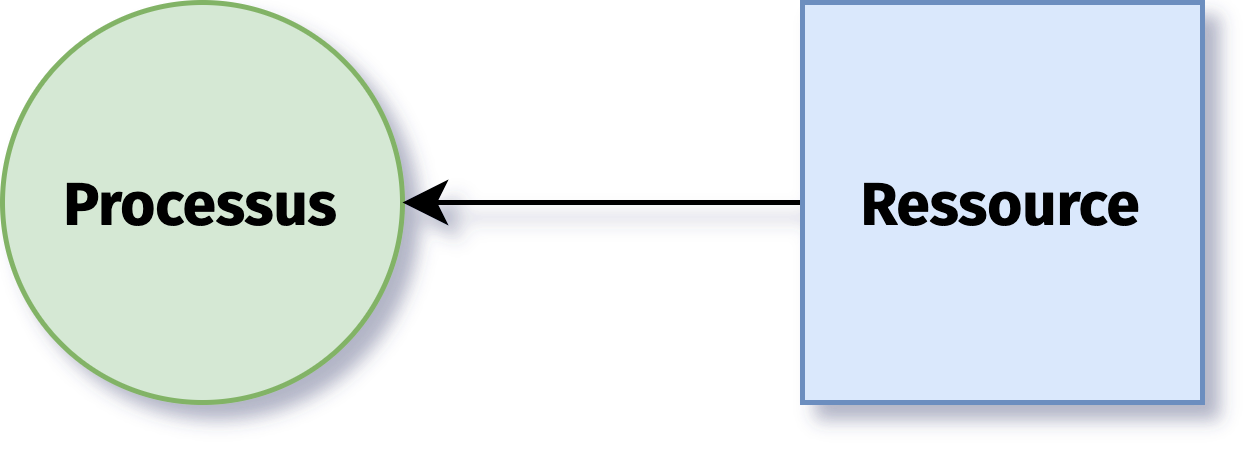
\includegraphics[width=5cm]{img/d1.png}
			\end{center}
	\item 	le ressource est détenue par un autre processus et donc le processus attend qu'elle soit libre et on représente cela ainsi :
	\begin{center}
			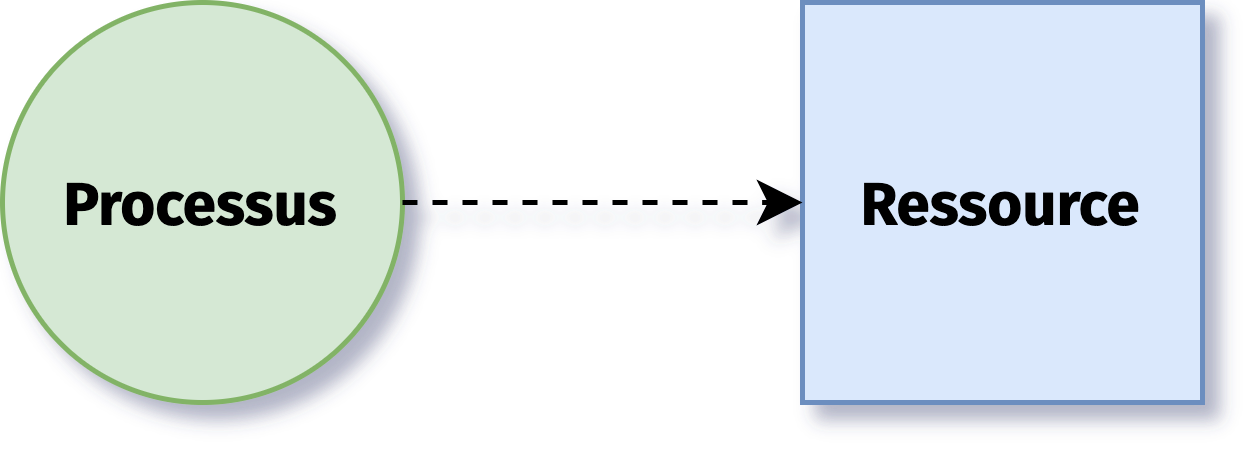
\includegraphics[width=5cm]{img/d2.png}
			\end{center}
\end{itemize}

\subsection*{Séance}

On va procéder ainsi

\begin{enumalph}
	\item Par groupe de 3, chacun choisit un processus qu'il va essayer d'exécuter.
	\item On dispose R1, R2 et R3 sur la table de jeu.
	\item À chaque tour, on lance un dé : sur un résultat de 1 ou 2 c'est P1 qui exécute une étape de son programme, 3 ou 4 pour P2 et 5 ou 6 pour P3.\\
	\item À chaque tour, on complète le graphe d'allocation.
	\item  Si pour une raison ou une autre les processus ne peuvent se terminer, indiquer pour quelle raison.
\end{enumalph}

L'objectif est de produire un scénario pour lequel les processus sont « bloqués » et de noter l'enchaînement des graphes d'allocation sur la fiche.


\end{document}